
\documentclass[11pt,a4paper]{article}
\usepackage[left=2cm,right=2cm,top=2cm,bottom=3cm]{geometry}
\usepackage{amsmath,amsfonts,amsthm,amssymb,varioref,times, commath}
\usepackage{gensymb}
\usepackage{tikz}
\usepackage{textcomp}
\usepackage{hyperref}
\hypersetup{
 colorlinks=true,
 linkcolor=blue,
 filecolor=magenta, 
urlcolor=cyan,
}
\usepackage{lipsum}
\usepackage{epigraph}
%to resume numbering in a list
\usepackage{enumitem}
%----- arrows 
\usepackage{extarrows}

%    differential equatiosn 
\usepackage{diffcoeff}   %\diff[2]{x}{y}


%%%%%%pour ecrire en français avec les accents
\usepackage[utf8]{inputenc}
\usepackage[T1]{fontenc}
\usepackage{lmodern} % load a font with all the characters
\usepackage{units}
%%%%%%%Image-related packages
\usepackage{wrapfig}
\usepackage{float, graphicx}
\graphicspath{ {./img/} }
\usepackage{subcaption}
\usepackage[export]{adjustbox}

%%%%%%%pour faire des cadres
\usepackage{xcolor}
\usepackage{tcolorbox}
\usepackage{framed}
\usepackage{mdframed}


%%%%%%%chemistry frmulae
\usepackage{chemfig}
\usepackage{chemformula}
\usepackage[version=4]{mhchem}

% -------------- Circuits -------------------
\usepackage[european, straightvoltages]{circuitikz}

% Title & headers
\usepackage[explicit]{titlesec}
% Raised Rule Command:
% Arg 1 (Optional) - How high to raise the rule
% Arg 2 - Thickness of the rule
\newcommand{\raisedrulefill}[2][0ex]{\leaders\hbox{\rule[#1]{1pt}{#2}}\hfill}
\titleformat{\section}{\Large\bfseries}{\thesection. }{0em}{#1\,\raisedrulefill[0.4ex]{1pt}}

% pour ecrire sur +sieurs colonnes
\usepackage{multicol}
\setlength{\columnseprule}{0pt}
\setlength{\columnsep}{60pt}
% Fusion de lignes de tableaux.
\usepackage{multirow}
% Position verticale des lettres dans la ligne de tableau.
\usepackage{array}

% physics -----------------------------------------------------------
\newcommand{\To}{\longrightarrow}
\newcommand{\gpl}{\; g\cdot L^{-1}}
\newcommand{\gpmol}{\; g\cdot mol^{-1}}
\newcommand{\mpl}{\; mol\cdot L^{-1}}
\newcommand{\mps}{\; m\cdot s^{-1}}
\newcommand{\rps}{\; rad\cdot s^{-1}}
\newcommand{\kph}{\; km\cdot h^{-1}}
\newcommand{\mpss}{\; m\cdot s^{-2}}
\newcommand{\Dt}{\Delta t}
\newcommand{\vv}{\vec{v}}
\newcommand{\va}{\vec{a}}
\newcommand{\vp}{\vec{p}}
\newcommand{\vf}{\vec{F}}
\newcommand*{\Vf}[1]{\overrightarrow{F_\ensuremath{{#1}}}}
\newcommand{\es}[1]{\cdot10^{#1}}
\newcommand{\eng}[1]{\textcolor{purple}{(= #1})}
\usepackage{harpoon}
%\newcommand*{\vect}[1]{\overrightharp{\ensuremath{#1}}}
\newcommand*{\Vect}[1]{\overrightarrow{\ensuremath{#1}}}
\newcommand{\pfd}[1]{\sum \vec{F}_{ext_{#1}} &= \od{\vp_{#1}}{t} = m\cdot\va_{#1}}
\newcommand{\C}{\degree C}
\newcommand{\Delt}{\Delta t}

% --- Circuits ------------
\newcommand{\bipole}[1]{
\begin{circuitikz} \draw
(0,0) to[ #1 ] (2,0); 
\end{circuitikz} {\hspace{5mm}}}

% Chimie ---------------------------------
\newcommand{\oxo}{\ce{H3O+}_{(aq)}}
\newcommand{\eau}{\ce{H2O}_{(\ell)}}
\newcommand{\OH}{\ce{HO-}_{(aq)}}
\newcommand{\AH}{\ce{AH}_{(aq)}}
\newcommand{\A}{\ce{A-}_{(aq)}}
\newcommand{\MnO}{\ce{MnO_4^{-}}}
\newcommand{\conc}[1]{\left[{#1}\right]}
\newcommand{\couple}[2]{\ce{#1/#2}}


% Environnements ------------------------
\newcounter{exo}
\newenvironment{exo}[1][]
{\refstepcounter{exo} \begin{shaded}\noindent $\triangleright \quad$\textbf{Exercice~\theexo. #1} } { \end{shaded}}
\newenvironment{eg}
{\begin{shaded} \textbf{Exemple:} } { \end{shaded}}

\newenvironment{defn}[1]
{\begin{leftbar}\noindent \textbf{Définition :\textit{ \quad #1}} } { \end{leftbar}}

%\newenvironment{rmrq}
%{\begin{shaded} \textbf{Remarque.\quad } \itshape } { \end{shaded}}
\newenvironment{rmrq}
{\begin{mdframed}[backgroundcolor=blue!10, linewidth=0pt] \textbf{Remarque.\quad } \itshape } { \end{mdframed}}

\newenvironment{python}
{\begin{shaded} \textbf{A faire en PYTHON}\\ \itshape } { \end{shaded}}

% Shading colour -----------------------------
\definecolor{shadecolor}{gray}{0.9}

\date{}
\author{}

\renewcommand*\contentsname{Résumé}









% Title & headers 
\usepackage{fancyhdr}
\pagestyle{fancy}
\fancyhf{}
\lhead{SciPhy : Terminale spé}
\rhead{$\chi $ - 6 : Electrolyse}
\chead{2020-28}
\rfoot{Page \thepage}
\lfoot{\textcopyright\; S Zayyani}
\renewcommand{\footrulewidth}{0.1pt}% default is 0pt

\title{\large Chimie - Chapitre 6 \\ \LARGE  L'électrolyse : évolution forcée d'un système chimique}
\date{}
\author{}

\setlength{\parindent}{0mm}
\setlength{\parskip}{2mm}

%%%%%%%%%%% For wrapfigure 
\setlength{\intextsep}{-5pt}%
\setlength{\columnsep}{10pt}%



\begin{document}
\maketitle
\vspace{-1cm}
\begin{tcolorbox}[title=Notions de la classe de première à rappeler]
oxydoréduction ; réaction chimique ; notions de base d'électricité
%\tcblower
\end{tcolorbox}
\tableofcontents


\section{Rappels}

\begin{wrapfigure}[2]{r}{0.25\textwidth}
\centering
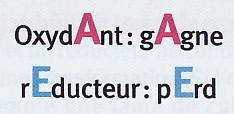
\includegraphics[width=0.95\linewidth]{imgs/c6/mnemo.jpg}
\end{wrapfigure}

Quelques définitions et notions à se rappeler : 
\begin{itemize}
    \item Un \textbf{oxydant} est une espèce chimique capable de \textbf{gagner} (ou capter) des électron 
    \item On dit que l’oxydant est réduit.  
    \item Une \textbf{réduction} est donc une \textbf{capture d’électrons}.
    \item Un \textbf{réducteur} est une espèce chimique capable \textbf{céder} (ou perdre) des électrons.
    \item On dit que lors de cette réaction le réducteur s’oxyde.  
    \item Une \textbf{oxydation} est donc une \textbf{perte d’électron}. 
\end{itemize}

Pour résumer : 
\begin{align*}
    \ce{Oxydant + n e- &->[reduction] Reducteur } \\
    \ce{Reducteur &->[oxydation] Oxydant + n e- }
\end{align*}      
\newpage
Le couple \textit{rédox} est donc défini : 
\begin{itemize}
    \item Une espèce oxydante et une espèce réductrice forment un couple oxydant/réducteur (Ox/Red) si l’on peut passer de l’une à l’autre par gain ou perte d’électron(s).
    \item Un tel couple est noté ox/red (l’oxydant noté toujours d’abord, à gauche). \item On parle donc d’oxydant et de réducteur conjugué.  
    \item on associe donc à un couple ox/red une demi-équation d’oxydoréduction (rédox) : $\ce{Ox + ne- = Red}$
\end{itemize}
Afin de trouver la demi-équation d'un couple rédox : 
\begin{mdframed}[backgroundcolor=red!5]
\begin{enumerate}
    \item Écrire l’ébauche de la demi-équation sans les coefficients stœchiométriques
    \item Équilibrer les atomes de l’élément commun à l’oxydant et au réducteur.
    \item Équilibrer les atomes d’oxygène en ajoutant des molécules d’eau  $\ce{H2O_{(\ell)}}$
    \item Équilibrer les atomes d’hydrogène avec les ions $\ce{H+_{(aq)}}$.
    \item Équilibrer les électrons en utilisant des électrons $\ce{e-}$.
\end{enumerate}
\end{mdframed}

\begin{rmrq}
\begin{itemize}
    \item Il est très important de noter que les transformations étudiées dans ce chapitre ont lieu en solution aqueuse, mais que comme les électrons libres ne peuvent exister en solution, cette écriture est formelle et constitue une schématisation.  
    \item Tous les électrons perdus par le réducteur sont donc captés par l’oxydant.  
    \item Lorsque la présence des ions $\ce{H+_{(aq)}}$ est nécessaire afin d’équilibrer la demi-équation, cela indique que la réaction a lieu dans un milieu acide (ou milieu acidifié).  
	\item Il y a bien un lien entre la structure électronique d’un élément, son placement dans la classification périodique et son caractère oxydant ou réducteur.  Les principaux réducteurs sont les métaux et les alcalins-terreux.  Les principaux oxydants sont les corps simples (en particulier le dioxygène), et les dihalogènes.  
\end{itemize}
\end{rmrq}

\subsection*{Réactions de rédox}
\begin{itemize}
    \item Une réaction d’\textbf{oxydoréduction}, aussi appelée une réaction \textbf{rédox}, est une réaction caractérisée par un transfert d’électrons entre deux réactifs : l’oxydant et le réducteur.  
    \item Il s’agit donc d’une réaction entre deux couple rédox.
    \item L’oxydant d’un couple réagit avec le réducteur de l’autre couple, et les produits de la réactions sont le réducteur et l’oxydant conjugués.
\end{itemize}

L’équation chimique rédox entre les couples $\ce{Ox_1 /Red_1}$ et $\ce{Ox_2 /Red_2}$ avec 
$\begin{cases}       
\ce{Ox_1 + n1e- = Red_1}\\
\ce{Ox_2 + n2e- = Red_2}
\end{cases}$:
\[\ce{n2 Ox1 + n1 Red2 -> n1 Ox2 + n2 Red1}\]

\section{Classification des couples rédox}
Jusqu'alors, en voyant deux couples rédox, nous n'avions pas d'idée quel oxydant (de quel couple) réagirait le réducteur de l'autre couple.  Par conséquent en regardant deux couples, par exemple $\couple{Zn^2+}{Zn}$ et $\couple{Ag+}{Ag}$, il existait deux réactions possibles : entre $\ce{Zn^2+}$ et $\ce{Ag}$, ou entre $\ce{Zn}$ et $\ce{Ag+}$. 

En réalité il n'y a qu'une seule réactionqui se produit \textit{de manière spontanée} à chaque fois entre ces deux couples: 

\[ \ce{2Ag+ + Zn -> 2 Ag + Zn^2+} \]

\begin{wraptable}[11]{r}{0.4\linewidth} 
\begin{rmrq} 
\small{Pour aller plus loin, à chaque couple rédox est associé un ``potentiel standard d'oxydoréduction'' qui est une mesure quantitative de cette puissance oxydative. Les valeurs sont exprimées en volts, et relatives à une valeur de $0$ attribuée au couple $\couple{H+}{H2}$. Une pile, constituée de deux demi-équations de deux couples rédox, génère une tension égale à la différence de potentiels standards des deux couples: $E_{pile} = E\degree_2 - E\degree_1$. } 
\end{rmrq} 
\end{wraptable}
En fait, tout oxydant n'est pas ``égal'', c'est à dire que certains oxydant sont ``plus oxydant'' que d'autres. C'est le cas ici de l'ion $\ce{Ag+}$ qui est plus puissant que l'ion $\ce{Zn^2+}$. On parle ici de la \textbf{puissance oxydative}, qui est une propriété naturelle des différentes espèces chimiques. 

La manière la plus simple de savoir quels sont les réactifs et les produits d'une réaction de rédox entre deux couples, est de placer les deux couples sur un axe verticale (le sens vers la haut pour la puissance croissante d'oxydation), et puis appliquer la ``règle du gamma'' (figure ci-après). 
\\
\begin{figure}[H]
\centering
\begin{subfigure}{.5\textwidth}
  \centering
  % include first image
  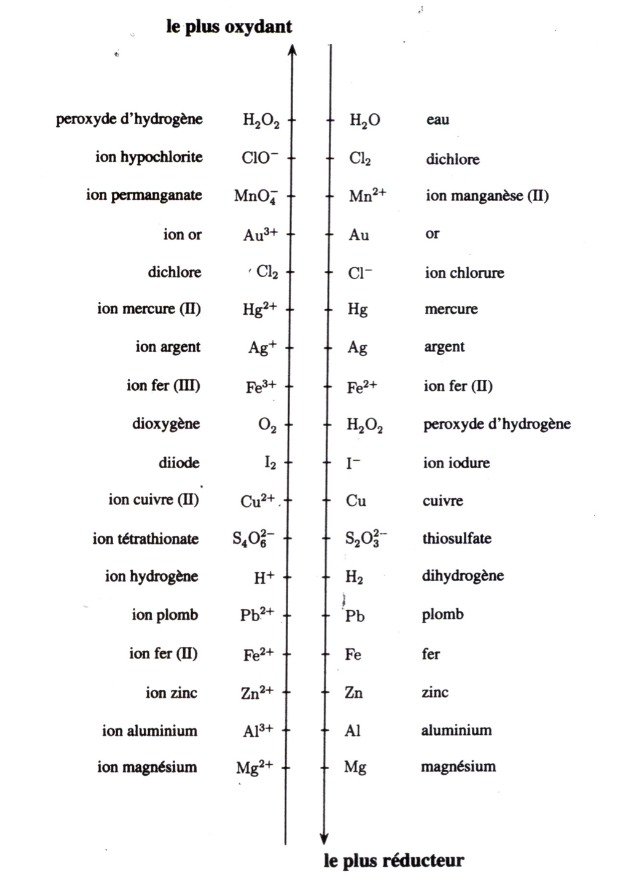
\includegraphics[width=\linewidth]{imgs/c6/classementoxydant.png}  
  \caption{classement des couples rédox en fonction de la puissance d'oxydation/réduction}
\end{subfigure}
\begin{subfigure}{.4\textwidth}
  \centering
  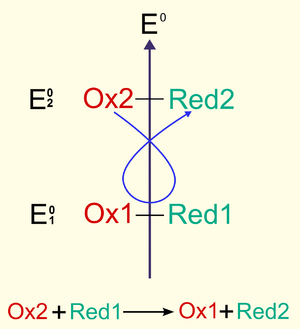
\includegraphics[width=\linewidth]{imgs/c6/gamma.png}  
  \caption{Application de la règle du gamma.}
\end{subfigure}
\end{figure}


\section{Électrolyse}
Il est très important de comprendre que tout ce que nous avons appris dans la partie précédente est bien le cas pour des réactions qui se produisent de \textit{manière spontanée}. Cela veut dire qu'elle se produisent sans un apport énergétique de notre part (plus ou moins si l'on veut être rigoureux). 

Il ne faut pas oublier le principe d'équilibre que nous avons déjà vu souvent (dans beaucoup de différents domaines) : un système tend naturellement vers un état d'équilibre. L'étude de la pile que nous avons fait dans un chapitre précédent est un très bon exemple de ce phénomène. Deux couples rédox mis-en-contacte qui spontanément produisent une réaction électrochimique. 

\begin{exo}
Y-a-t-il une réaction si : 
\begin{itemize}
    \item On plonge une lame de fer dans une solution de nitrate d'argent? 
    \vspace{1.5cm}
    \item on plonge une lame d'argent dans une solution d'acide chlorhydrique? 
    \vspace{1.5cm}
    \item on plonge une lame de magnésium dans une solution de chlorure de nickel (II) ? 
    \vspace{1.5cm}
\end{itemize}
\end{exo}


\subsection{Réactions non-spontanées}

Est-il alors possible de ``forcer'' une réaction qui ne peut pas avoir lieu spontanément? Serait-il possible, par exemple, de forcer une réaction entre l'argent métallique et l'ion de zinc? 

Faisons un raisonnement ensembles : Nous avons déjà établi qu'une pile est une réaction d'oxydoréduction spontanée, et qui génère une tension (jusqu'à ce que les réactifs s'épuisent). Mais il y a des piles que nous utilisons dans des appareils, comme des téléphones portables, qui se vident en journée et que l'on ``recharge'' pendant la nuit, pour réutiliser le lendemain; et on les recharge en les branchant sur une prise de secteur; \textbf{autrement dit on les recharge en leur appliquant une tension électrique}.  

Cette recharge n'est pas possible sans qu'on \textbf{force} cette tension sur la batterie. Voilà donc la réponse à notre question du départ : Il existe des systèmes susceptibles de subir une transformation, sans qu'ils évoluent de manière spontanée. \textbf{Dans le cas des réaction d'oxydoréduction, une telle transformation non-spontanée ou forcée s'appelle l'électrolyse. }

\subsection{Principe de l'électrolyse}

\begin{defn}{Électrolyse\eng{electrolysis}}
\begin{itemize}
    \item Lors d'une électrolyse, un \textbf{générateur électrique impose un transfert d'électrons} correspondant à une transformation qui n'aurait pas lieu spontanément. 
    \item L'électrolyse est une \textbf{transformation forcée}. 
    \item Pour qu'une électrolyse puisse se produire, il faut que la tension imposée par le générateur soit supérieure à celle de la réactions d'oxydoréduction spontanée (correspondant à la différence des potentiel standard des couples mise-en-jeu). 
\end{itemize}
\end{defn}

L'électrolyse a lieu dans un appareil nommée un \textbf{électrolyseur}. L'électrolyseur est constitué d'une cuve remplie d'une solution électrolytique. Les deux électrodes baignant dans la solution sont reliées aux bornes du générateur. 

C'est au niveau des électrodes qui se produisent les deux demi-équation rédox correspondant à la réaction entre les deux couples:
\begin{itemize}
    \item L'\textbf{Anode} le siège de  l'\textbf{oxydation}
    \item La \textbf{Cathode} le siège de la \textbf{réduction}. 
\end{itemize}

\begin{mdframed}[backgroundcolor=red!2]
A la cathode la réaction est la réduction de l'oxydant le plus fort. 

A l'anode la réaction est l'oxydation du réducteur le plus fort. 
\end{mdframed}

\begin{exo}
Justifier le fait que l'anode est lié au pôle + du générateur, et la cathode au pôle -. 
\vspace{3.5cm}
\end{exo}

\begin{figure}[H]
\centering
\begin{subfigure}{.43\textwidth}
  \centering
  % include first image
  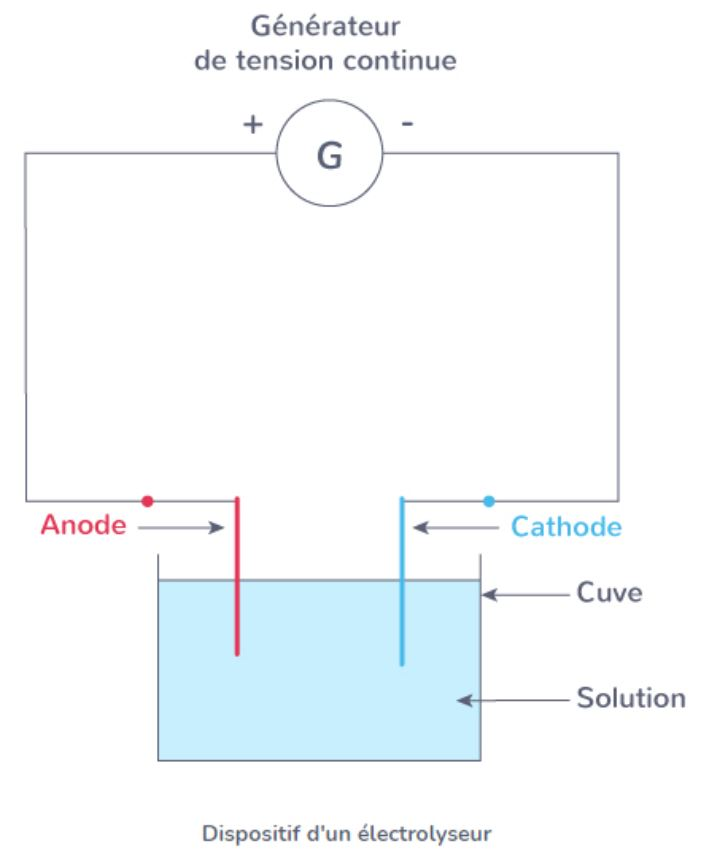
\includegraphics[width=.95\linewidth]{imgs/c6/electrolyseur.jpg}  
\end{subfigure}
\begin{subfigure}{.54\textwidth}
  \centering
  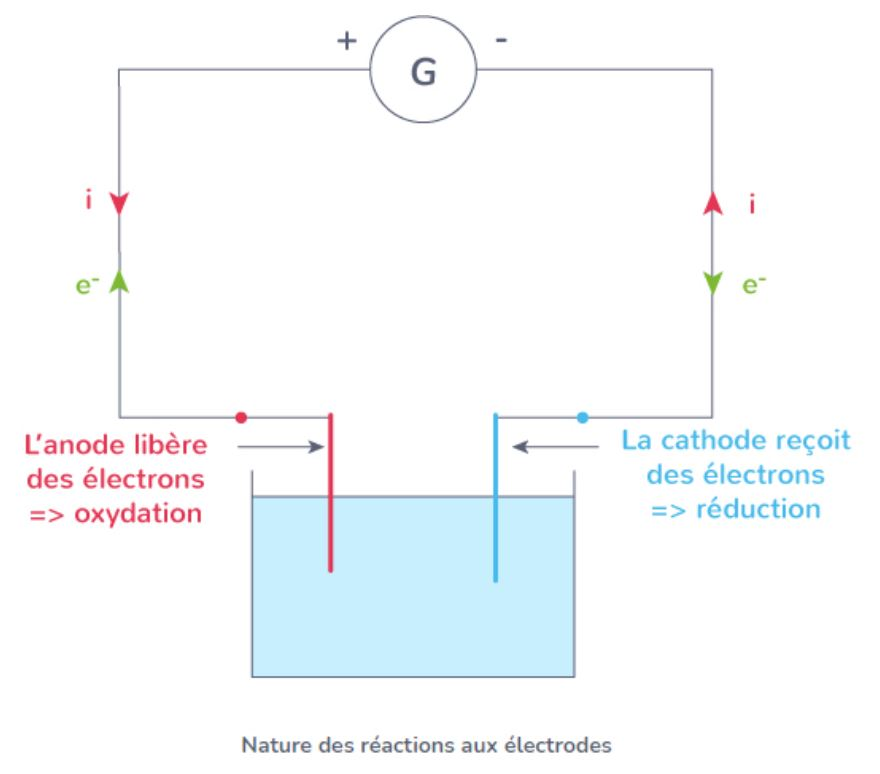
\includegraphics[width=.95\linewidth]{imgs/c6/anodcatho.jpg}  
\end{subfigure}
\end{figure}
 \newpage
\subsection{Réactions forcée \& constante d'équilibre}

Comme nous avons déjà vu, nous pouvons expliquer et décrire l'électrolyse grâce aux notions du quotient et de la constante de réaction. Une réaction spontanée va toujours dans le sens qui va pousser le quotient de la réaction vers la constante de la réaction. Il va de soi donc qu'une électrolyse, n'étant pas spontanée, va transformer les quantités des matières des réactifs et des produits dans le sens qui éloigne le quotient de la réaction de la constante $K$. Tant que le générateur impose sa tension, le système électrochimique reste hors de l'état de l'équilibre. 

%EXO AVEC QUOTIENTS.....

\section{Etude quantitative}

Il est très facile de mesurer la quantité de charge électrique échangée lors d'une réaction d'électrolyse. Il suffit de mesure l'intensité du courant $I$ et la durée $\Dt$ et nous avons : 
\[Q=I\cdot \Dt \tag{1}\]
De plus, nous connaissons la charge d'un électron $\ce{e-}$, et la nature de la réaction d'oxydoréduction qui a lieu, nous pouvons alors déterminer exactement les quantités de matières disparue ou formé lors de l'électrolyse. Le lien entre tout cela est la \textbf{constante de Faraday} $\mathcal{F}$, qui est la \textbf{charge d'une mole d'électron}. Par définition $\mathcal{F} = 96500\;C$. 

La charge totale $Q$ transférée pendant une électrolyse, dépend donc du nombre de mole d'électrons échangé $n_{\ce{e-}}$ : 
\[ Q = n_{\ce{e-}}\cdot\mathcal{F} \tag{2}
\]
d'après (1) et (2) nous avons : 
\begin{align*}
    Q &= I\cdot \Dt = n_{\ce{e-}}\cdot\mathcal{F} \\
    \Longleftrightarrow n_{\ce{e-}} &= \dfrac{I\cdot\Dt}{\mathcal{F}} \tag{3}
\end{align*}

Et donc, de manière générale pour une demi-équation $\ce{aA + n e- -> bB }$ où l'on met l'avancement $x = n$ :
\[ \dfrac{n_{\ce{e-}}}{x} = \dfrac{n_A}{a} = \dfrac{n_B}{b}
\]

\begin{eg}

\begin{wrapfigure}[7]{r}{0.3\linewidth}
\centering
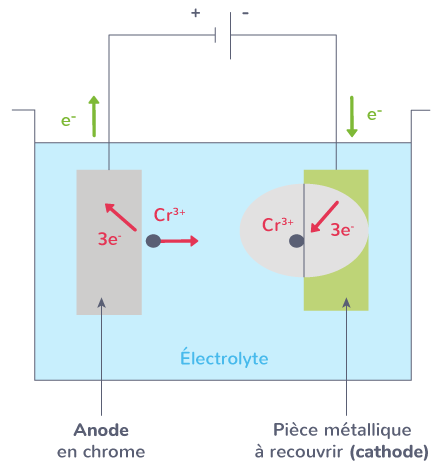
\includegraphics[width=0.95\linewidth]{imgs/c6/chrome.png}
\end{wrapfigure}

Il est une pratique de se servir d'électrolyse pour recouvrir un métal d'un autre métal. Considérer le cas où l'on veut couvrir une plaque métallique de chrome. Comme dans la figure suivante, la cathode sera le métal que l'on couvrir de chrome, baigné dans une solution contenant des ions $\ce{Cr^3+}$, et une plaque en chrome comme anode. 

Les réactions qui auront lieux : 
\begin{itemize}
    \item Anode (oxydation) : $\ce{Cr_(s) = Cr^3+ + 3 e-}$
    \item Cathode (réduction) : $\ce{Cr^3+ + 3 e- = Cr_(s)}$
\end{itemize}
La réaction rédox est donc : $\ce{Cr_(s) + Cr^3+_{(aq)} <=> Cr_(s) + Cr^3+_{(aq)}} \tag{1}$
Pour recouvrir l'anode, il faut un courant d'intensité $I$ pendant une durée $\Dt$. La quantité de charge échangée est donc : 
\[ Q = I\cdot\Dt = n_{\ce{e-}}\cdot\mathcal{F} \tag{2}\]
D'après la réaction (1) donc : 
\[ \dfrac{n_{\ce{e-}}}{3} = \dfrac{n_{\ce{Cr}}}{1} \Longleftrightarrow n_{\ce{e-}} = 3 n_{\ce{Cr}}  \]
et donc avec (2) : 
\[ n_{\ce{Cr}} = \dfrac{I\cdot\Dt}{3\cdot\mathcal{F}}\]
ce qui donne une masse de chrome : 
\[ m_{\ce{Cr}} = \dfrac{I\cdot\Dt}{3\cdot\mathcal{F}}\cdot M(\ce{Cr})\]
\end{eg}
Considérons un autre exemple, un peu plus complexe. 

\begin{eg}

\begin{wrapfigure}[9]{r}{0.35\linewidth}
\centering
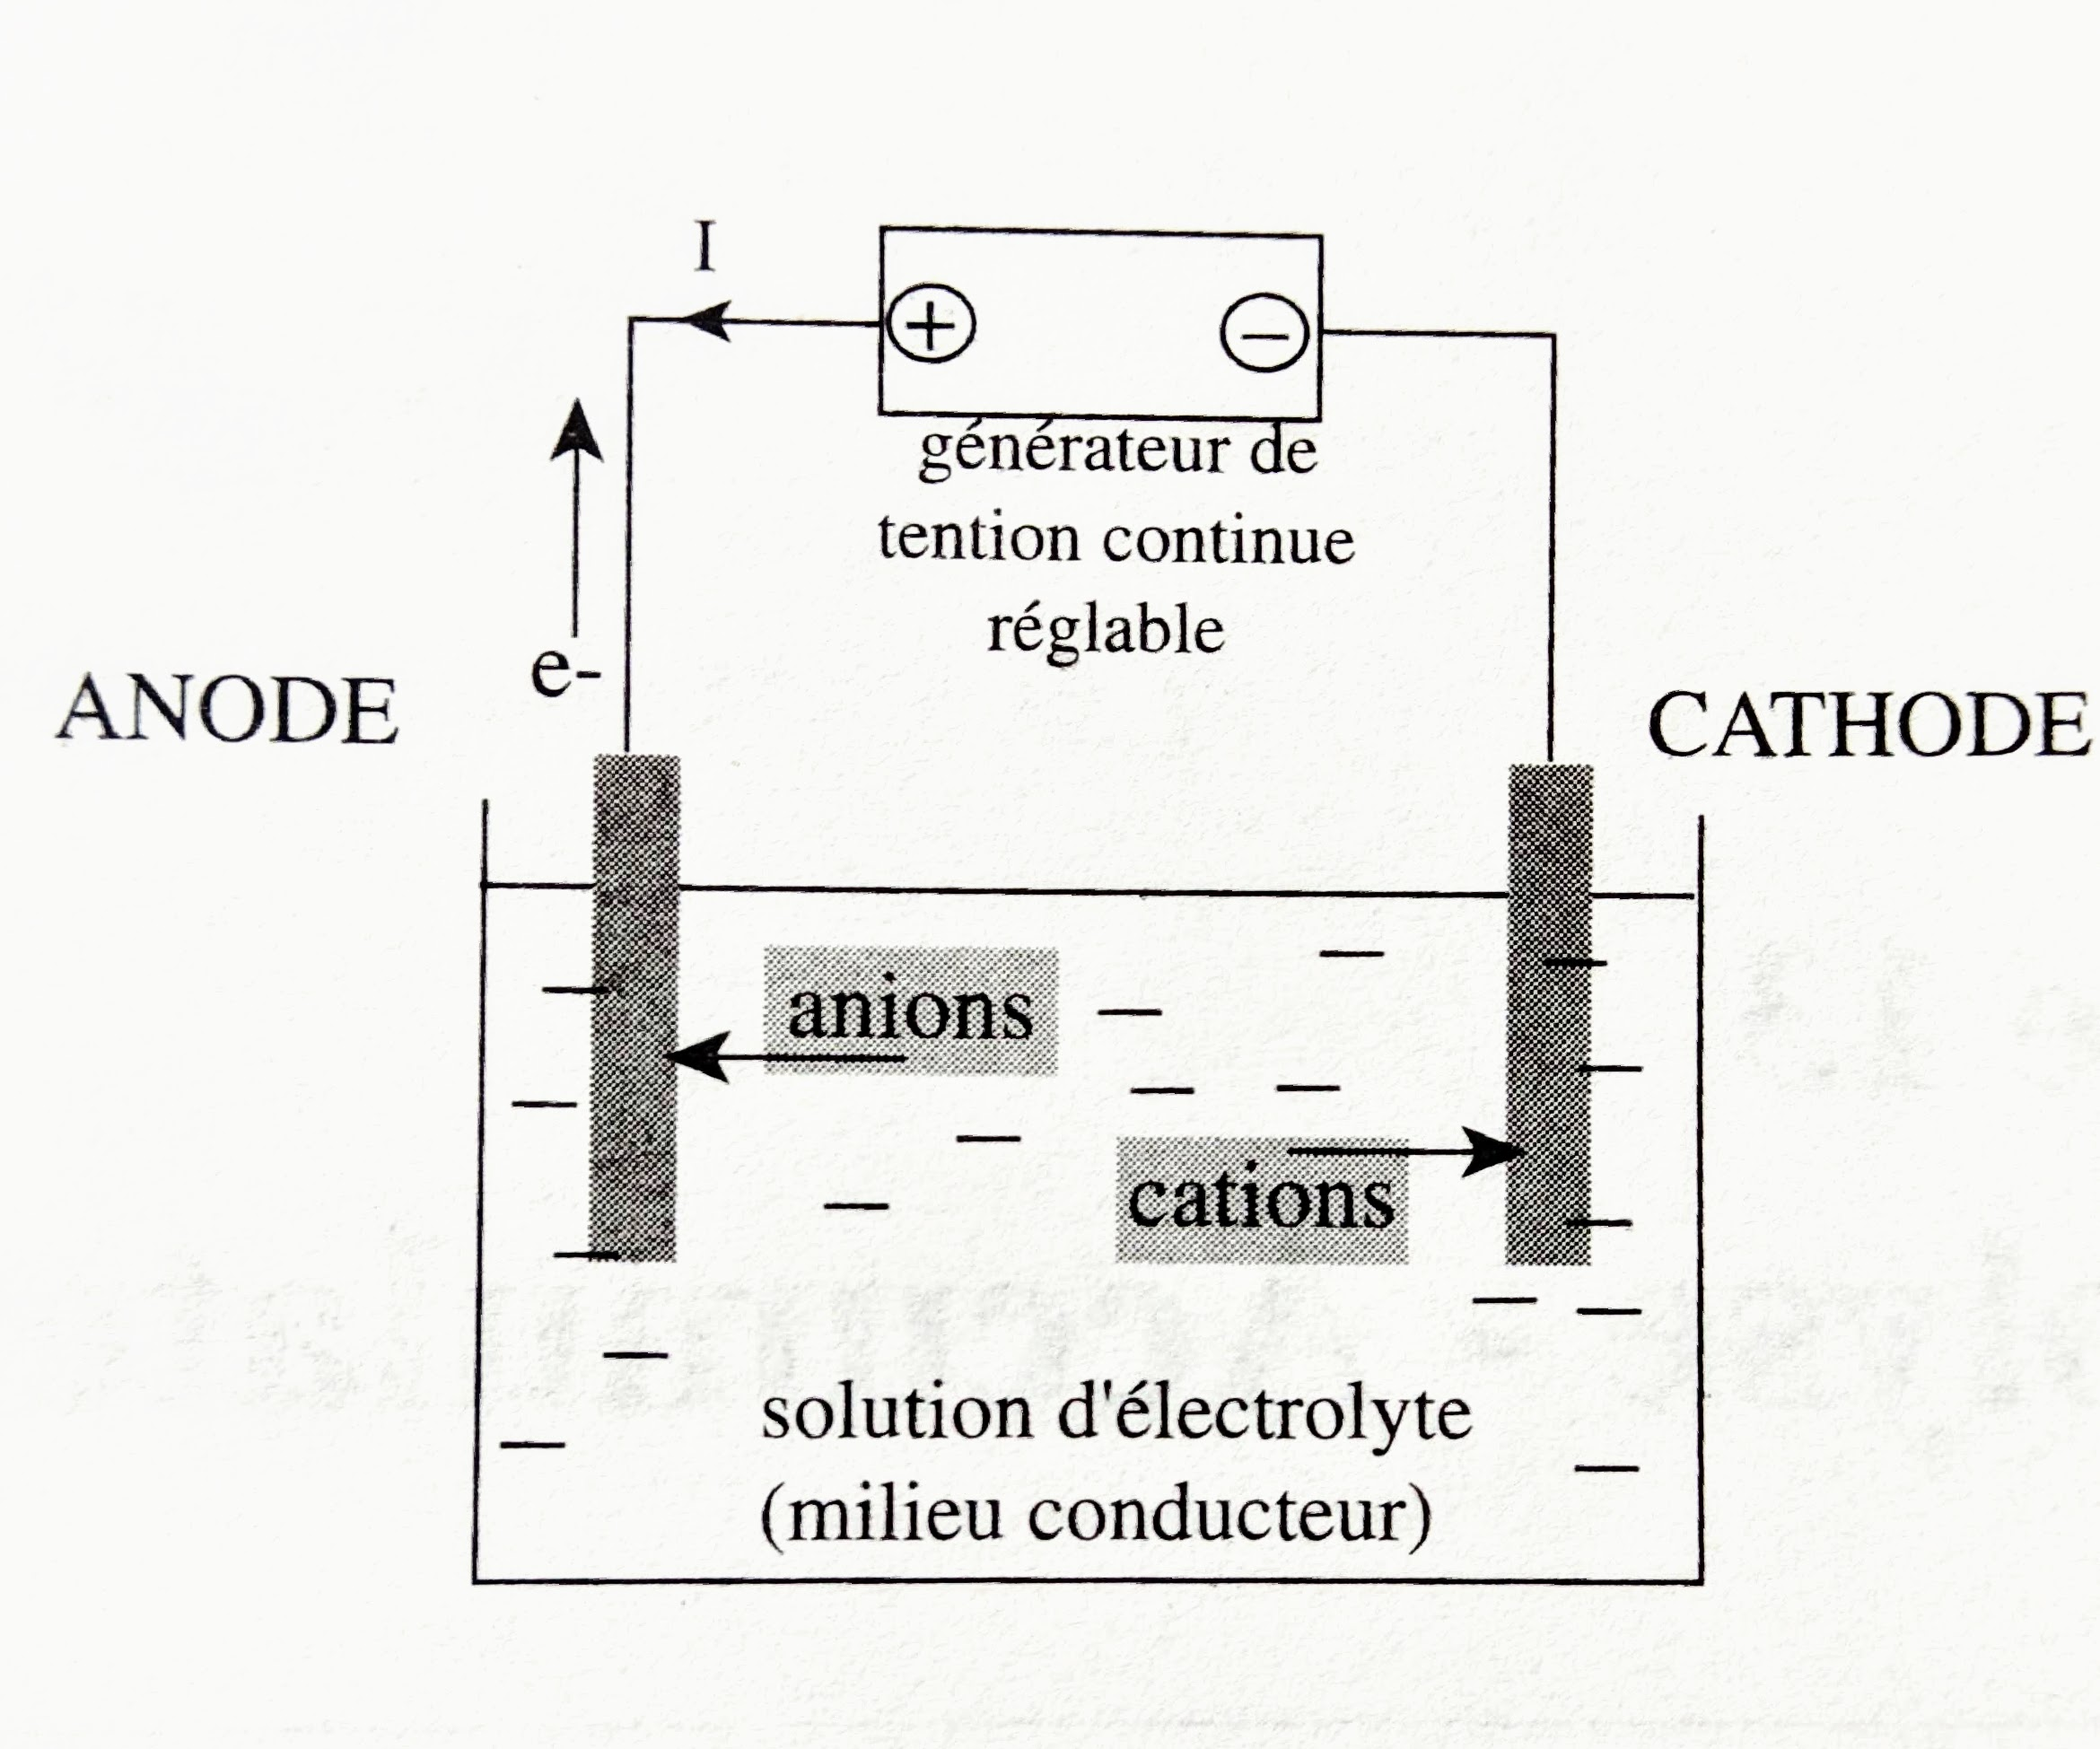
\includegraphics[width=0.95\linewidth]{imgs/c6/exosulfate.jpg}
\end{wrapfigure}

On réalise l'électrolyse d'une solution de sulfate de cuivre (II) (acidifié par de l'acide sulfurique) avec des électrodes en graphite. Voici donc le schéma de l'électrolyse : 

Les couples rédox qui sont potentiellement en jeux sont (dans l'ordre décroissant de puissance de l'oxydant) : $\ce{S2O8^2- / SO4^2-} \quad , \quad \ce{O2 /H2O}\quad , \quad  \ce{Cu^2+/Cu}\quad , \quad \ce{H+/H2} $

Les espèces présentes dans l'électrolyseur sont $\ce{H2O }, \ce{Cu2+}, \ce{SO4^2-}$. Les réactions donc qui peuvent se produire aux électrodes : 
\begin{multicols}{2}
\begin{itemize}
    \item Anode (oxydation) : 
    \begin{itemize}
        \item $\ce{H2O -> O2 + 4H+ + 4e-} $
        \item $\ce{2SO4^2- -> S2O8^2- + 2e-} $
    \end{itemize}
    \item Cathode (réduction) :
    \begin{itemize}
        \item $\ce{2H+ + 2e- -> H2}  $ (car milieu acide)
        \item $ \ce{Cu2+ + 2e- -> Cu_(s)}$    \end{itemize}
\end{itemize}
\end{multicols}

Mais il faut déterminer la réaction qui a effectivement lieu à chaque électrode. Cela se fait selon le principe précédemment énoncé : à la cathode la réduction se fait avec l'oxydant le plus fort, et à l'anode l'oxydation se fait avec le réducteur le plus fort. 

Et donc les réactions qui ont lieu effectivement : 
\begin{multicols}{2}
\centering
\textbf{Anode} : $\ce{H2O -> O2 + 4H+ + 4e-} $\\
\textbf{Cathode} : $ \ce{Cu2+ + 2e- -> Cu_(s)}$ 
\end{multicols}

Et donc la réaction globale : $ \ce{2Cu2+ + H2O -> O2 + 4H+ + 2Cu_(s)}$ 
C'est à dire qu'on doit observation la formation d'un gaz, le dioxygène, au niveau de l'anode, et la cathode en graphite se recouvre en cuivre. 

On applique un courant de $8\; A$ pendant 30 minutes. On voudrait déterminer la masse de cuivre, et le volume de dioxygène qui se formera. 

A partir de la relation (3) : $n_{\ce{e-}}= \dfrac{I\Dt}{\mathcal{F}}$

\begin{multicols}{2}
A l'anode  : 
\begin{align*}
    n_\ce{O} &= \dfrac{1}{4} n_{\ce{e-}} \\
    V_\ce{O} &= n_{\ce{O}} \cdot V_M \\
    &= \dfrac{8\cdot 1800}{4\cdot 96500}(22,4) = 0,83\;L
\end{align*}

A la cathode  :  
\begin{align*}
    n_\ce{Cu} &= \dfrac{1}{2} n_{\ce{e-}} \\
    m_\ce{Cu} &= n_{\ce{Cu}} \cdot M(Cu) \\
    &= \dfrac{8\cdot 1800}{2\cdot 96500}(63,5) = 4,74\;g
\end{align*}
\end{multicols}
\end{eg}

\textbf{On peut se poser la question} : Que se passerait-il si l'une des électrodes n'était pas inertes, et était en cuivre par exemple?

Dans ce cas-là, comme vous pourriez le justifier vous-même, la réaction qui aura lieu sera $\ce{Cu -> Cu^2+ + 2e-}$. Ce qui se passe alors est la transformation du cuivre métal, en ion cuivre à l'anode, et conversion de l'ion cuivre en métal cuivre à la cathode, c'est à dire un transport du cuivre depuis l'anode vers la cathode, entraînant une disparition de l'électrode en cuivre au bout d'une certaine durée. 

\begin{exo}
Disposant d'une solution aqueuse de sulfate d'argent, on voudrait argenter une électrode en métal, et une électrode inerte. Les couples mise-en-jeu sont (ordre décroissant de puissance d'oxydant) :
$$\ce{O2 /H2O}\quad , \quad \ce{Ag+/Ag}\quad , \quad \ce{SO4^2- / SO2} \quad , \quad \ce{H+/H2}  $$ 
\begin{enumerate}
    \item Faire un schéma légendé du montage. 
    \item Trouver les réactions possibles à chaque électrode.
    \item Donner la réaction qui se produit à chaque électrode. 
    \item La surface à argenter est $s=0,25\;m^2$. L'épaisseur de la couche est $e=0;015\;mm$. La densité de l'argent est $d=10,5$. Si le générateur fournit un courant de $I=60\;A$, combien de temps $\Dt$ l'électrolyse doit-elle durer?
\end{enumerate}
\vspace{7cm}
\end{exo}

\section{Accumulateurs \& d'autres applications}

\begin{wrapfigure}[8]{r}{0.5\linewidth}
\centering
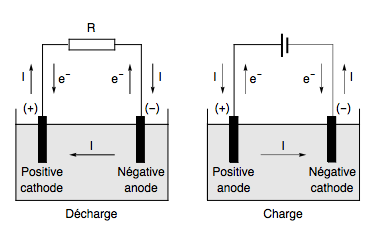
\includegraphics[width=0.95\linewidth]{imgs/c6/accumul.png}
\end{wrapfigure}

\begin{defn}{Accumulateur\eng{Rechargable battery}}
\begin{itemize}
    \item Il s'agit d'un dispositif électrochimique capable de se comporter comme : 
    \begin{itemize}
        \item \textbf{Récepteur : } Il se comporte comme un électrolyseur. Il reçoit l'énergie électrique d'un générateur et ``se charge''. 
        \item \textbf{Générateur : } Il se comporte comme une pile. Il fournit son énergie au circuit en ``se déchargeant''. 
    \end{itemize}
\end{itemize}
\end{defn}

Il existe de nombreux exemples d'accumulateurs dans nos vies quotidiennes : 
\begin{itemize}
    \item Les batteries utilisées dans les appareils électroniques portables (ordinateurs, téléphone, lecteur mp3, etc.) sont des accumulateurs ``Lithium-ion''. 
    \item Les batteries utilisées dans les voitures (depuis près d'un siècle) sont des accumulateurs au plomb. 
\end{itemize}

% \begin{exo}
% Un accumulateur au plomb est constitué de deux électrodes en plomb dans une solution aqueuse d'acide sulfurique et de sulfate de plomb (II). L'une des électrodes est recouverte de dioxyde de plomb. Les couples mis-en-jeux sont $\ce{PbO2_{ (s)} / Pb^2+_{ (aq)}}$ et $\ce{Pb^2+ / Pb_{ (s)}} $ 
% \end{exo}

\end{document}